\documentclass[sigconf]{acmart}
%\usepackage{booktabs} % For formal tables
\usepackage{times}
\usepackage{helvet}
\usepackage{courier}
\usepackage{amsmath}
\usepackage{graphicx}
\usepackage{subfigure}
\usepackage{amssymb}
%\frenchspacing
%\setlength{\pdfpagewidth}{8.5in}
%\setlength{\pdfpageheight}{11in}
%\pdfinfo{
%/Title (Modeling Trajectory as Image)
%/Author (Jianming Lv)
%}
\pagestyle{empty}                   %������ҳüҳ��
\setcounter{secnumdepth}{0}
 \begin{document}
% The file aaai.sty is the style file for AAAI Press
% proceedings, working notes, and technical reports.
%
\title{Modeling Trajectory as Image: Convolutional Neural Networks for Multi-scale Taxi Trajectory Prediction}
%\author{Jianming Lv\\
%School of Computer Science and Engineering, South China University of Technology\\
%Guangzhou, 510006, China\\
%}
\nocite{*}
\begin{abstract}
Precise destination prediction of Taxi trajectories can benefit both efficient schedule of taxies and accurate advertisement for customers.In this paper, we propose T-CONV, a novel trajectory prediction algorithm, which models trajectories  as two-dimensional images and utilize multi-layer convolutional neural networks to extract multi-scale spatial patterns for high prediction accuracy. Compared with the traditional algorithms which process trajectories as one-dimensional sequences of spatial points, the image based model of T-CONV is easier to capture two-dimensional local spatial features of trajectories in different scales. Furthermore, in order to solve the sparsity problem of trajectories, we integrate multiple local convolutional fields in T-CONV to capture important specific areas of trajectories. Comprehensive experiments based on real trajectory data show that T-CONV can achieve much better results than state-of-the-art methods.
\end{abstract}

\keywords{Trajectory, Convolutional Neural Network, Multi-scale}

\maketitle

\section{Introduction}

Taxi has become one of the major transportation tools in big cities nowadays. For efficient schedule and security monitoring of taxis running in a city, the mobile GPS devices are broadly installed in most of taxis, which report the real-time trajectories of passengers to the supervise department.

Analysis of the destinations of taxi trajectories can benefit a lot interesting applications, such as intelligent schedule of taxis and accurate advertisement. For example, if a taxi company knows exactly the destination of a running taxi, it can efficiently dispatch the demands near the destination to the taxi. Another example is about the taxi TV advertising, which shows advertisements in the displays deployed in taxis for passengers. Good understanding of the target of a trip may be helpful for making  proper recommendation for different passengers,e.g. showing  film posters in the taxi going to a cinema. However, most of the time, taxi drivers operating with an electronic dispatch system do not indicate the final destination of their current ride, so it is necessary to predict the destination of a running taxi based on historical trajectories.

%On the other hand, if an advertisement company understands the destination of a passenger, e.g. a cinema, it can push some advertisement highly related to the destination such as some posts of newest films to the TV installed on the taxi.

The recent event most related to this prediction problem is the ECML-PKDD competition \cite{kaggle2015}, which is set up to predict the destinations of taxi trajectories in Porto. The research \cite{de2015artificial}, which adopts MLP (multi-layer perception) and RNN (recurrent neural network) algorithms, wins the championship. Besides, recently proposed models \cite{xue2013destination,xue2015solving,citation-0}predict destination  by using Markov models to match query trajectories with historical records. \cite{chen2015predicting} clusters the moving objects according to their trajectories and make prediction according to the mobility patterns of similar objects.


Most of existing researches model trajectories as  sequences of spatio-temporal points and process them in one single spatial scale. This kind of one-dimensional data structures are hard to explicitly reveal the two-dimensional spatial features of trajectories, e.g. curves, crossings, corners, and windings. These patterns are highly related to the structure of road networks, and may benefit better understanding of the state and destination of taxi trajectories.  Furthermore, we address that trajectories have distinct multi-scale properties.  In a micro scale, a trajectory can be observed with precise positions, while it is hard to discover the global trend of large spatial scope. On the contrast side, in a macro scale, the global trend of a trajectory can be easily revealed, while many details are lost to support accurate prediction. The combination of the patterns in different scales may capture the motion features more precisely and completely for better prediction.

In this paper, we propose a novel prediction algorithm, T-CONV, which models trajectories from a different view to consider them as two-dimensional images and applies a multi-layer convolutional neural network (CNN)  to extract  multi-scale trajectory features for accurate prediction. Comprehensive experiments based on the real data of the ECML-PKDD contest\cite{kaggle2015} show that our model can achieve much better precision than the state-of-the-art algorithms.

The main contributions of this paper are summarized as follows:

\begin{itemize}
\item Different from traditional methods modeling trajectories as sequences of spatio-temporal points, we model trajectories as images and treat each spatio-temporal point as a pixel of the images. This model can transfer the multi-scale modeling methods, which are generally applied in image processing, to trajectory processing.
\item To our knowledge, this is the first time to deploy convolutional neural networks to combine multi-scale trajectory features to perform trajectory prediction. The multi-layer convolution and pooling operations enable T-CONV to extract multi-scale patterns from trajectories.
\item In order to solve the sparsity problem of trajectories, we integrate multiple local convolutional fields in T-CONV to capture important specific areas of trajectories. Compared with the traditional CNN  applied in image processing \cite{lecun1998gradient,krizhevsky2012imagenet}, which performs convolution on global images, T-CONV selects  multiple informative sub-areas as convolution fields to overcome data sparsity.
\item To analyze the effectiveness of T-CONV clearly, we also deploy the deconvolutional method\cite{zeiler2014visualizing} to visualize the patterns captured by T-CONV in different scales. Experiments show that T-CONV can learn small-scale trajectory patterns effectively in its lower convolutional layers and combine them into large-scale patterns in higher layers.

\end{itemize}

%The following sections are organized as follows. Section II describes some related work in this field. Section III offers some  preliminaries about the multi-scale property of trajectories. Section IV presents the main components of T-CONV. Section V shows experimental results to validate T-CONV. We conclude in the Section VI.

\section{Related Work}
In this section, we will introduce some research related to trajectory prediction.

Most of the existing researches model a trajectory as a one-dimensional spatio-temporal sequence and predict the destination by matching the query trajectory with historical trajectories. Specifically, \cite{krumm2006predestination,wei2012constructing,ziebart2008navigate} represents the map as a two-dimensional grid in a unified and fixed spatial scale, and all spatial points in one cell are considered as one location identified by the id of the cell. In this way, each trajectory can be modeled as a sequence of cell ids. These algorithms apply the Bayesian inference method to measure the probability of a given destination conditioned on the observed partial trajectory according to the statistics of the historical records. However, in real deployment, the sparsity problem of trajectories often makes it hard to find the historical trajectories exactly matching the query one. Simply adopting Bayesian inference as \cite{krumm2006predestination,wei2012constructing,ziebart2008navigate}   may return zero probability for all candidate destinations most of the time. To solve this problem, \cite{xue2013destination,xue2015solving}  decompose trajectories into sub-trajectories connecting two adjacent locations, and adopt first-orders Markov model to infer the probability of  all candidate destinations. \cite{citation-0}  extends the model to consider the difference between destinations and passing-by locations by adopting a absorbing Markov chain model. \cite{kim2007path}  utilizes the road network information and divides trajectories into road segments. The research aims to predict the future path of  a moving object by matching the query trajectory with historical trajectories on a road network.  \cite{chen2010system}  expresses a personal trajectory as a sequence of cells in a grid, and organize movement patterns in a pattern tree to support prediction.


Furthermore, clustering algorithms are commonly used techniques to overcome the sparsity problem and extract meaningful basic units in trajectories. \cite{chen2015predicting} clusters the moving objects according to their trajectories and makes prediction using the mobility patterns of similar objects.\cite{besse2016destination} clusters historical trajectories and uses the Gaussian mixture model to describe the distribution of spatial points in a trajectory cluster. Each query trajectory is assigned to multiple clusters and the mean of the destinations of these clusters is the predicted destination. \cite{alvarez2010trip} uses clustering algorithms to extract some important spatial points, named the support points, which are close to crossroads on trajectories. A HMM based algorithm is adopted to establish the relationship between support points and destinations. \cite{yang2014predicting} proposes a variant of the DBSCAN clustering algorithm to obtain stay points, and apply the variable order Markov Model to predict next locations of personal trajectories.

More recently, some neural network based algorithms \cite{de2015artificial} are proposed to accurately predict destinations of taxi trajectories and win the championship of the ECML-PKDD competition \cite{kaggle2015}.  \cite{de2015artificial} considers the first k points from the start and the last k points close to the end of a query trajectory, and feeds these spatial points into neural networks to  perform prediction. A lot of neural networks are test in the research, including normal multi-layer perception, LSTM\cite{hochreiter1997long}  based RNN(recurrent neural network), bi-directional RNN, and memory networks. Experiments based on a large validation set show that the bi-directional RNN outperform other methods.

Most of above studies perform prediction based on the trajectory features extracted in one specific spatial scale. In the grid based models \cite{krumm2006predestination,wei2012constructing,ziebart2008navigate,xue2013destination}, the scale is determined by the density of the grid, which is usually predefined and unified in the systems. The clustering  based algorithms \cite{chen2015predicting,besse2016destination,alvarez2010trip,yang2014predicting} cluster the spatial points and trajectories based on their spatial distribution and perform the prediction based on the clusters, which form a kind of specific spatial scale and  keep unchanged during the prediction. On the other hand,  neural network based models\cite{de2015artificial}, trajectories are processed in  a finest granularity and prediction is conducted based on the spatial points, each of which is represented as a tuple of latitude and longitude.

\section{Preliminaries}
\subsection{Multi-scale Patterns of Trajectory}

In this section, we analyze the multi-scale property of trajectories, and show the possibility of combining multi-scale trajectory features to achieve better understanding of motion patterns.

Fig.~1 illustrates a typical example of taxi trajectories in different scale. The dash line represents the query trajectory, which is used to predict the future destination of a taxi. 'O' is the start location of this taxi.  Fig.~1(a) shows the original trajectories. While processing trajectories in different scales, the grid is a commonly used tool to divide the map and combines the spatial points belonging to a same cell into one indivisible unit. Fig.~1(b) shows the micro-scale with dense grid, in which trajectories are recorded with fine granularity. Each trajectory is composed of a sequence of sampled points. In this scale, the view of trajectories display most details of their motion patterns, and the overlapping degree of the trajectories are low, which causes the sparsity problem when performing trajectory matching.  As we divide the map into a sparser grid, we can illustrate trajectories in a larger spatial scale as Fig.1(c). In this scale, the overlapping of the trajectories increases and the global trend of moving objects are easier to be captured. The trajectories are grouped into the two clusters, according to which the destination of the query trajectory may be 'x' with large probability. The Fig.1(d) illustrates a macro-scale, in which the global trend of trajectories is clearer and all trajectories overlap, but no detail of the local difference which may be important for accurate prediction is reserved.

\begin{figure}
\centering
\subfigure[]{
\begin{minipage}[b]{0.2\textwidth}
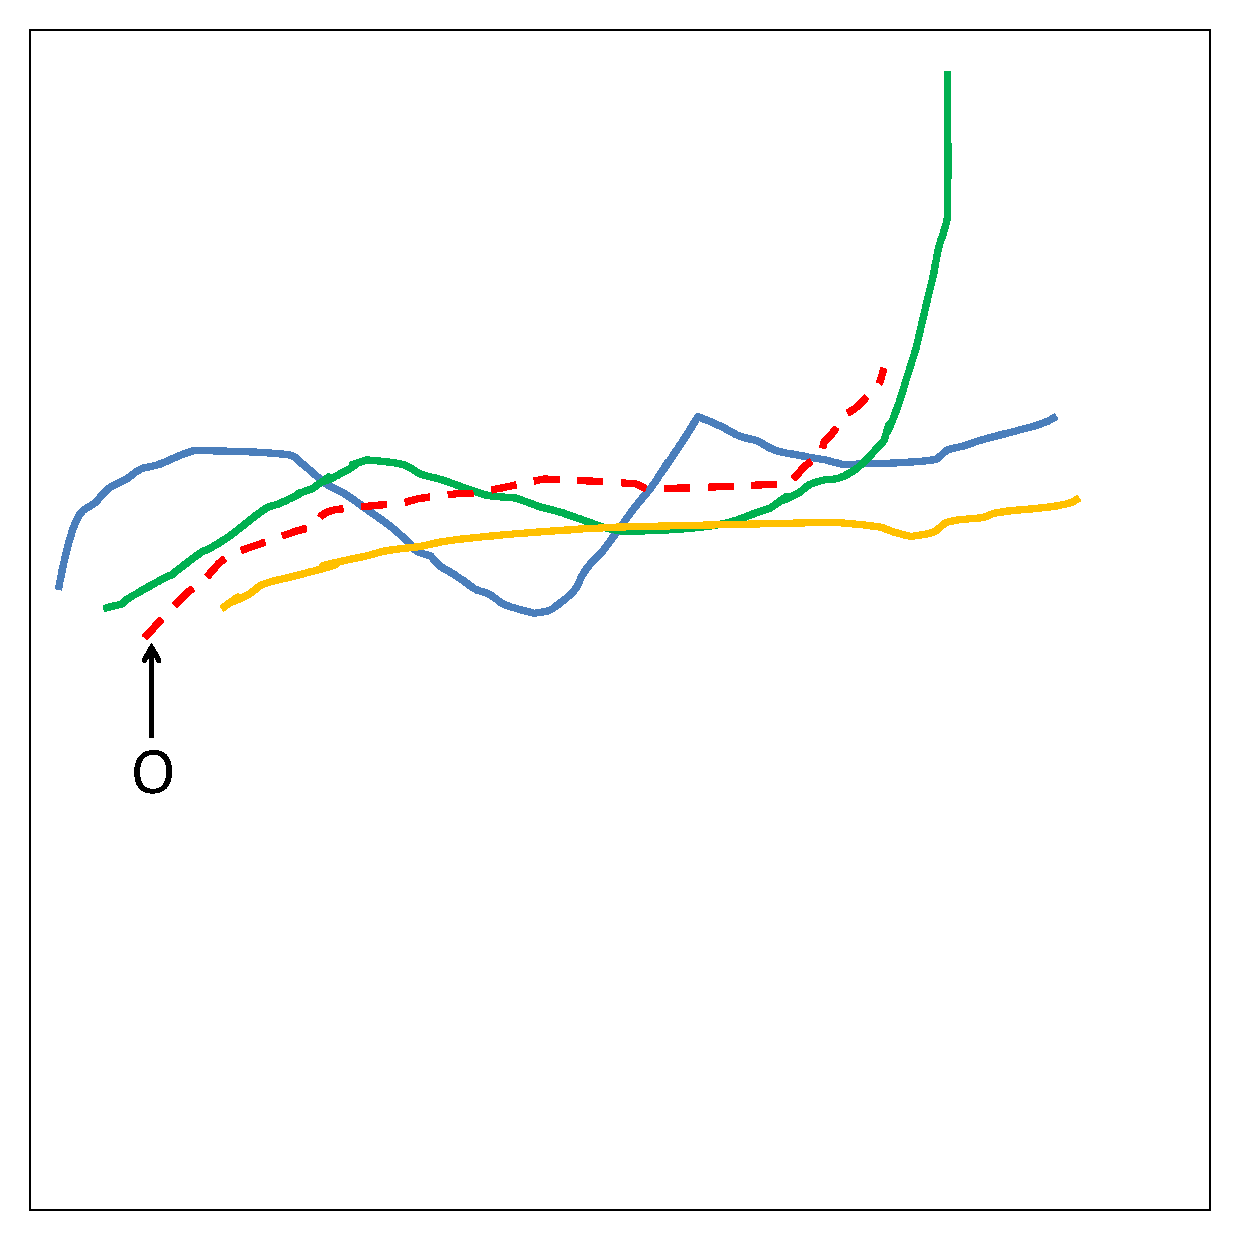
\includegraphics[width=1\textwidth]{./fig/Doc1.pdf}
\end{minipage}
}
\subfigure[]{
\begin{minipage}[b]{0.2\textwidth}
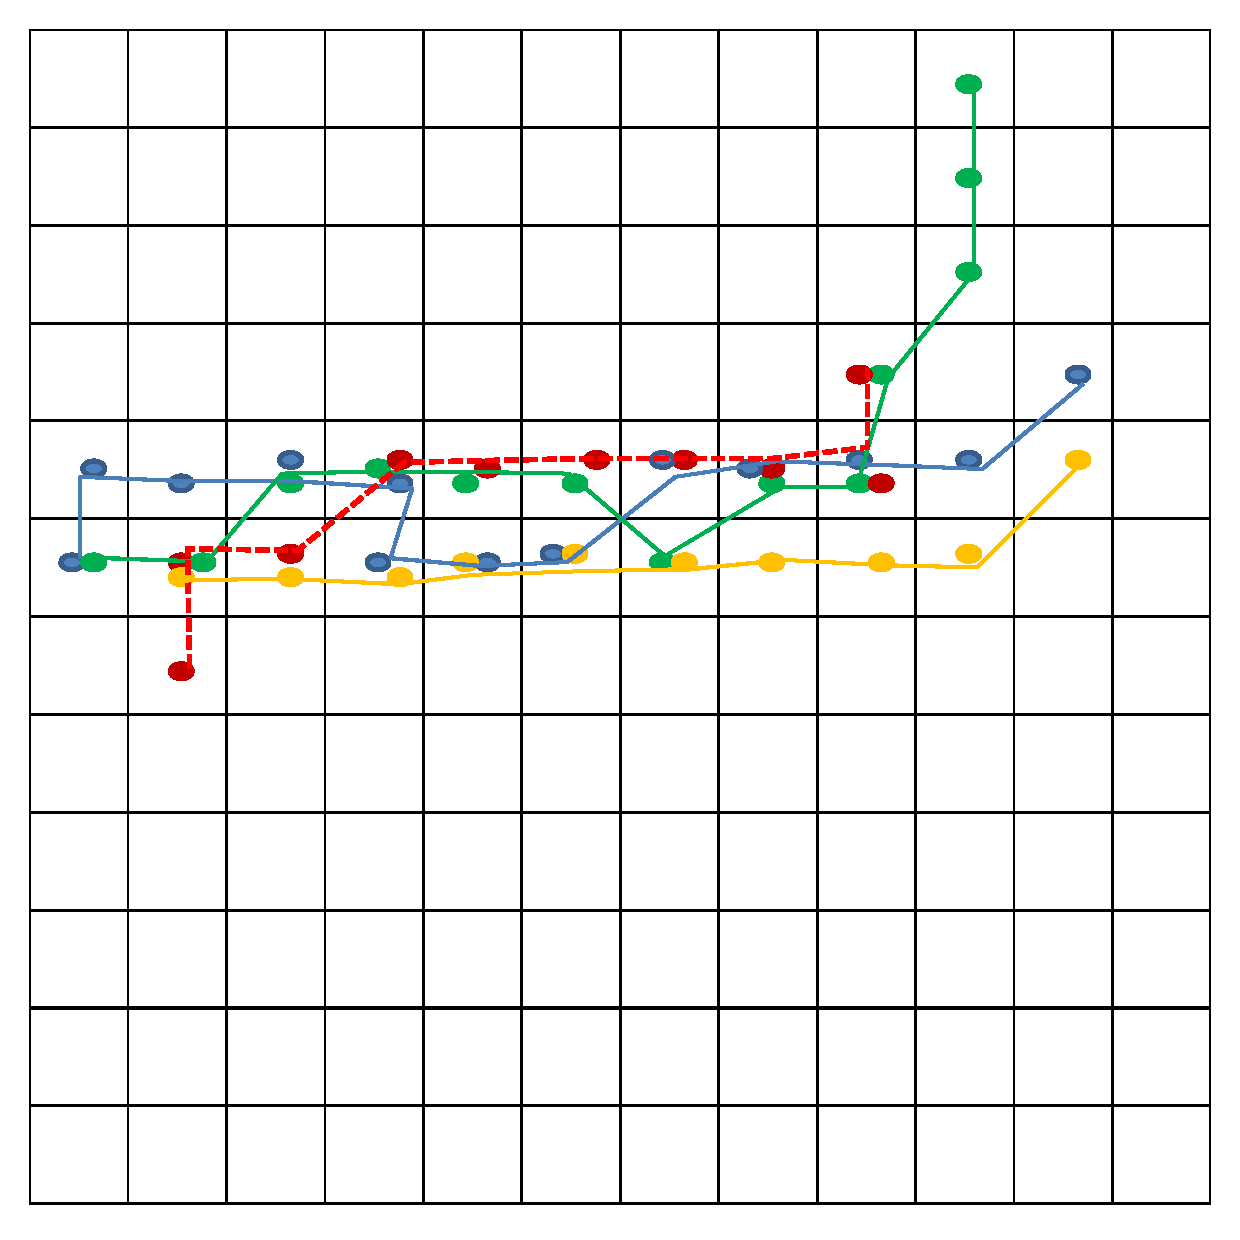
\includegraphics[width=1\textwidth]{./fig/Doc2.pdf}
\end{minipage}
}
\subfigure[]{
\begin{minipage}[b]{0.2\textwidth}
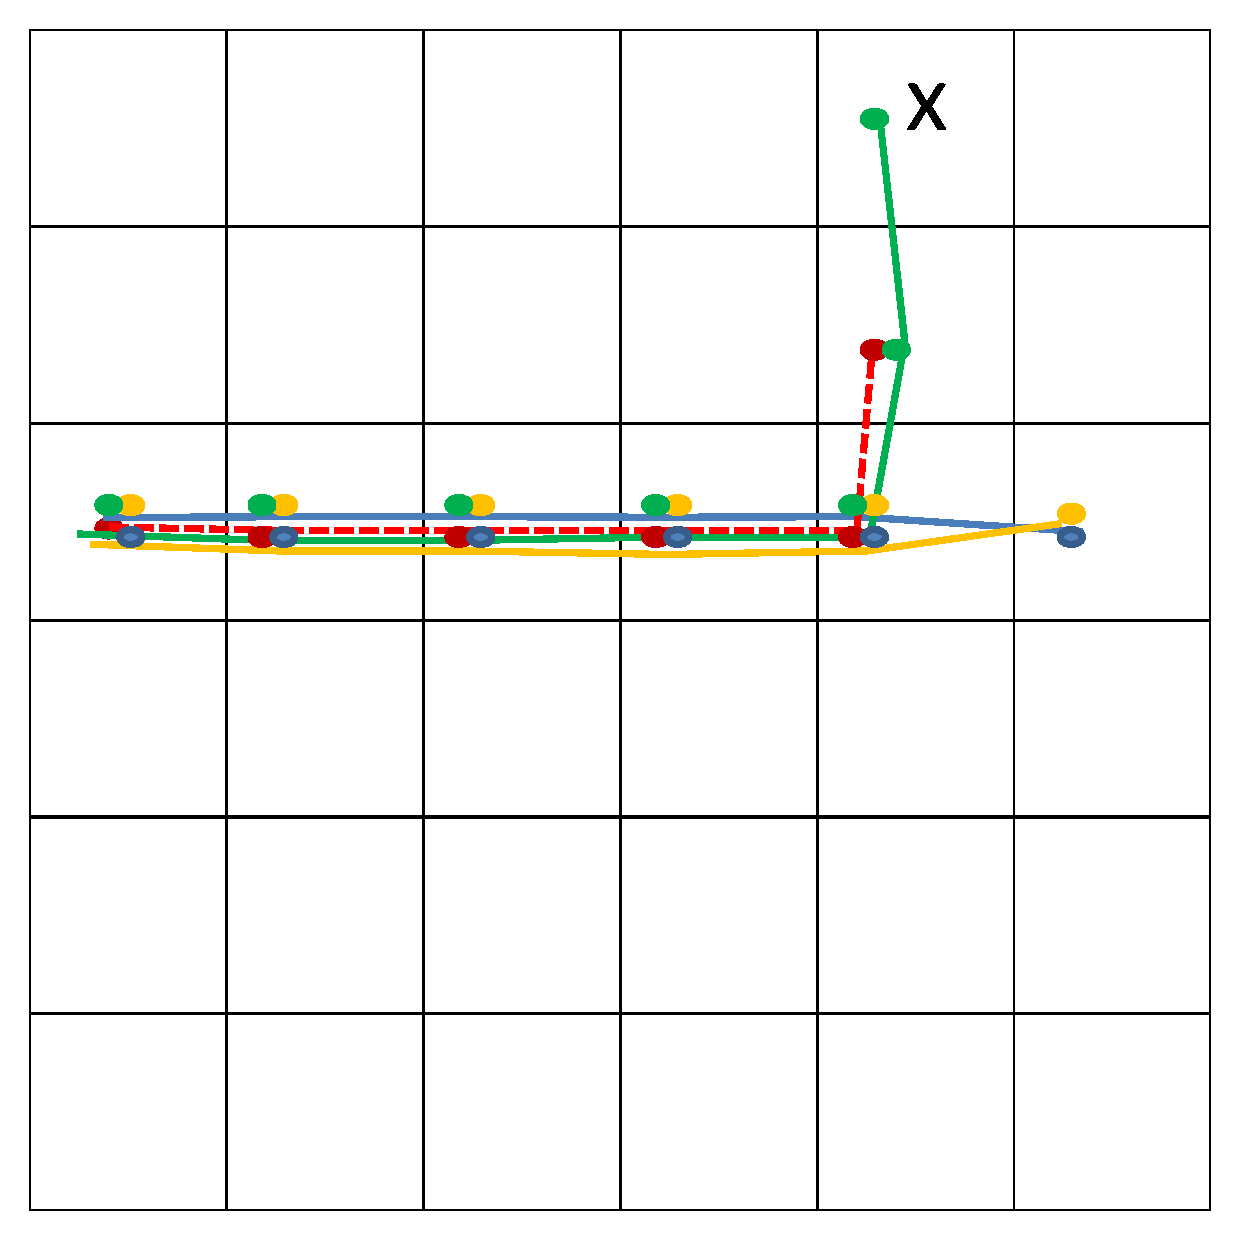
\includegraphics[width=1\textwidth]{./fig/Doc3.pdf}
\end{minipage}
}
\subfigure[]{
\begin{minipage}[b]{0.2\textwidth}
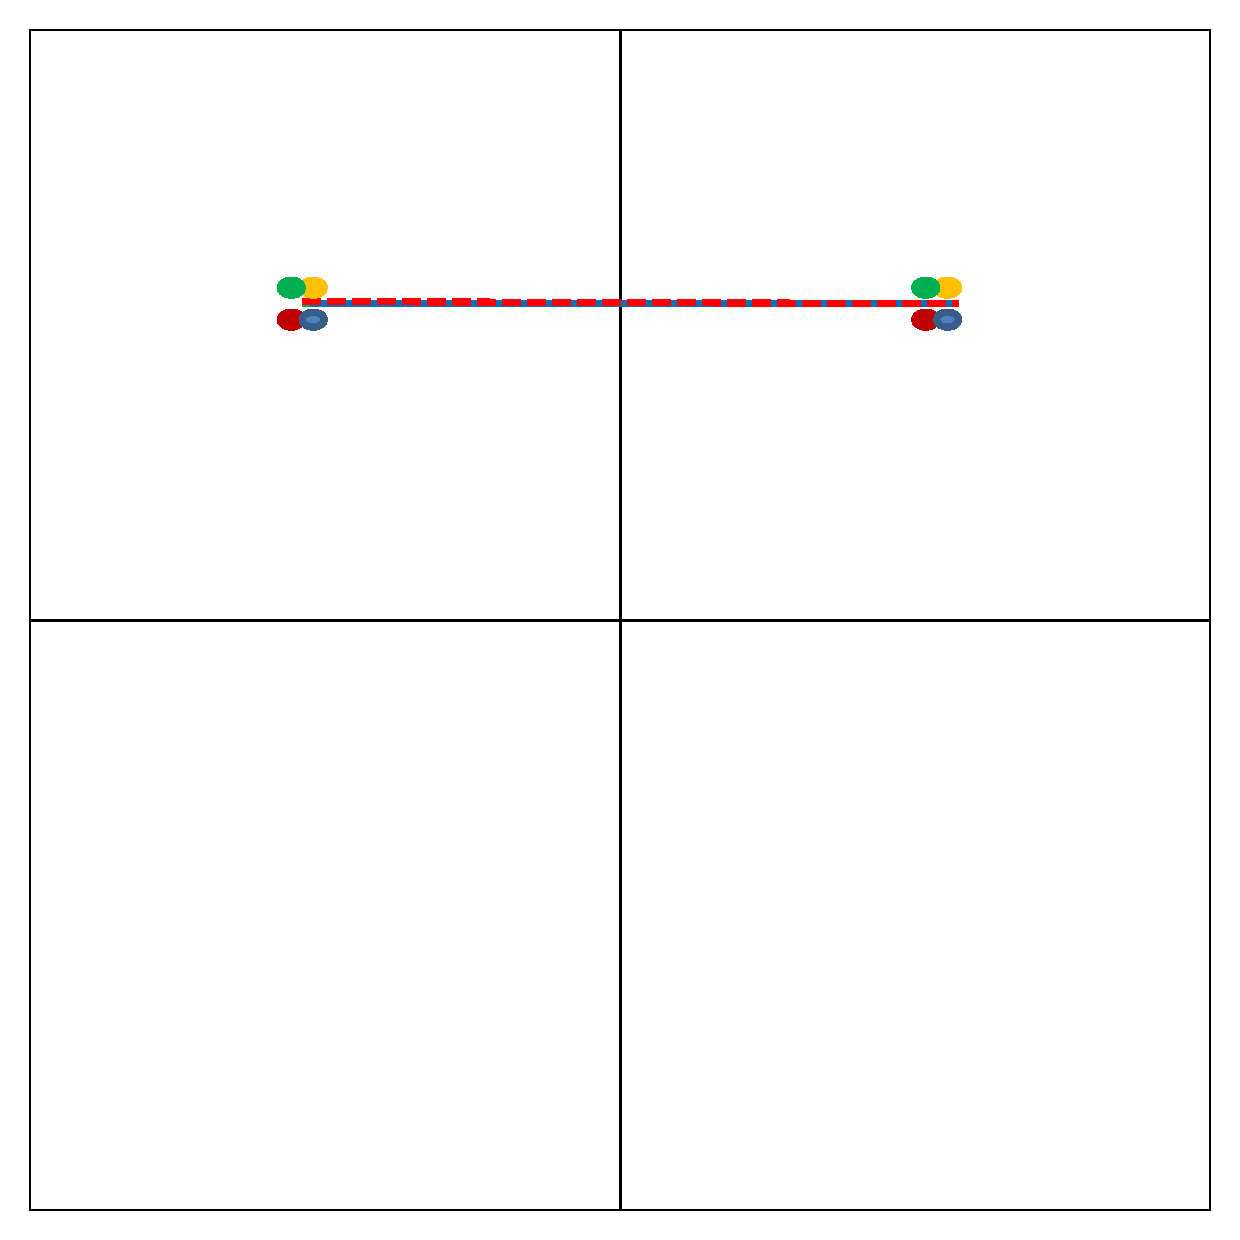
\includegraphics[width=1\textwidth]{./fig/Doc4.pdf}
\end{minipage}
}
\caption{Trajectories in different spatial scale.}
\end{figure}




In a word, trajectories in small scale show micro local motion patterns but cause sparsity problem, while in macro scale they show global trend clearly but it is difficult to sense important local  changes. The combination of the trajectory patterns in multiple scale may be better than the existing single scale based methods to capture both of the micro and macro motion patterns for more accurate prediction.


\section{T-CONV Models}
\subsection{Image Based Modeling of Trajectory}

Most of the traditional trajectory processing algorithms model a trajectory as a sequence of spatial points like:
\begin{eqnarray}
T_k = \{P_{k1},P_{k2},...\}.
\end{eqnarray}
Here  $P_{ki}(i \geq 1)$ is a GPS point of the trajectory. This one-dimensional data structure cannot explicitly reveal the intrinsic two-dimensional local spatial structures of trajectories as showed in Fig.~1(a),  including  corners, curves, crossings, and windings, which are important patterns to understand the evolving trend of a trajectory and support precise prediction.

In order to efficiently integrate the two-dimensional spatial features of trajectories, we model trajectories as images from different view. Like most of the grid-based preprocessing methods\cite{xue2013destination,krumm2006predestination,wei2012constructing,ziebart2008navigate}  of trajectories, we divide the map into a $M*M$ grid evenly as Fig.1(b), where $M$ is a predefined constant which denotes the highest resolution of the map. We use  $C_{mn}(1 \leq m,n \leq M)$ to denote the cell in the row $m$ and column $n$ of the grid. By mapping a trajectory $T_k$ on the grid,  each GPS point $P_{ki}$ is assigned to a cell $C(m, n)(1 \leq m,n \leq M)$. In this way, we can  achieve a two-dimensional $M*M$ image $I_k$, where the value of the pixel $I_k(m , n)(1 \leq m,n \leq M)$ indicates the information about the GPS points assigned to the cell $C_{mn}$.  The image  $I_k$ is called as the \emph{trajectory image} of $T_k$ in this paper. The detailed definition of the pixel value is presented in the following sections. Different from traditional one-dimensional sequence based modeling of trajectory, the trajectory image illustrates more directly the distribution of the spatial points on the two-dimensional map.

Based on this image based presentation of trajectories, the prediction problem can be formalized as follows: given a trajectory image $I_k$ of a running taxi starting from $P_{k1}$, it is required to predict the latitude and longitude of the destination of  the taxi.

\subsection{Global CNN for Trajectory Prediction}
The convolutional neural networks (CNN) based algorithms\cite{lecun1998gradient,krizhevsky2012imagenet}  are widely deployed recently to classify image accurately. CNN can be trained to extract multi-scale features from pixels level raw data of images by multi-layer convolution and max-pooling operations. Intuitively, we can transfer the successful deployment of CNN on images to process trajectory images.

Fig.~2 illustrates the architecture of the model, which deploys CNN over the global trajectory image. The model is named as \emph{\textbf{T-CONV-global}} in this paper.

The input of T-CONV-global is a $M*M$ trajectory image $I_0$.  Here $M$ is set to 30 in this example. Given any taxi trajectory $T_k = \{P_{k1},P_{k2},...,P_{kt}\}$, the value of each pixel $I_0(m,n)$ of the trajectory image is assigned as follows:

\[I_{0}(m,n)=\begin{cases}
0&\text{ if $ \nexists  i (1 \leq i \leq t \wedge P_{ki} \in C_{mn} )$ } \\
1&\text{ if $P_{kt} \in C_{mn} $ }\\
0.5&\text{ otherwise }
\end{cases}\]

Here $I_0(m,n)$ is set to 0 when the trajectory is not overlapped with the cell $C_{mn}$. Otherwise, $I_0(m,n)$ is set to a positive number. Specifically, it is set to 1 when the last point $P_{kt}$ of the trajectory is in $C_{mn}$, and it is set to 0.5  in other cases. The non-zero pixels show the curve of the trajectory, and  the difference between the last points and others indicates the direction of the trajectory.

As showed in Fig.~2, the convolution operations \cite{lecun1998gradient,krizhevsky2012imagenet}  are performed on $I_0$ to generate upper layer feature map $I_{11}$. Each 5*5 sliding window on $I_0$ are  mapped into one value in $I_{11}$ by a convolution kernel. After processing all of the sliding windows on $I_0$, a 26*26 matrix can be obtained, which is called one feature map. By applying multiple convolution kernels on $I_0$ , we can achieve multiple feature maps, e.g. 20 feature maps in this example. The main contribution of the convolution operations is to extract the local spatial dependency among neighboring spatial points.

The following max-pooling operations\cite{lecun1998gradient,krizhevsky2012imagenet}  down-sample each feature map in  $I_{11}$ to obtain a smaller one in  $I_{12}$ by filtering out the pixels with less activation values in each $t*t$ neighboring zone, where $t$ is called the pooling size. In this example, $t$ is assigned as 2. Each pixel value in  $I_{12}$  represents a local pattern of $t*t$ area in the trajectory image. Thus, each feature map in $I_{12}$  indicates an abstraction of the original image in a larger scale.

The combination of the convolution and max-pooling operations can be applied to the feature maps multiple times to form a hierarchical CNN.  Higher-level features exhibit the patterns in larger scale, which are calculated from the combination of lower-level features in smaller scale. In this way, multi-scale patterns are embedded in the output features of the highest level of CNN.  In this example, the convolution operations are applied twice, and the top layer $I_{22}$ consists of 50 feature maps with the size 4*4.

\begin{figure}
\centering
{
\begin{minipage}[b]{0.5\textwidth}
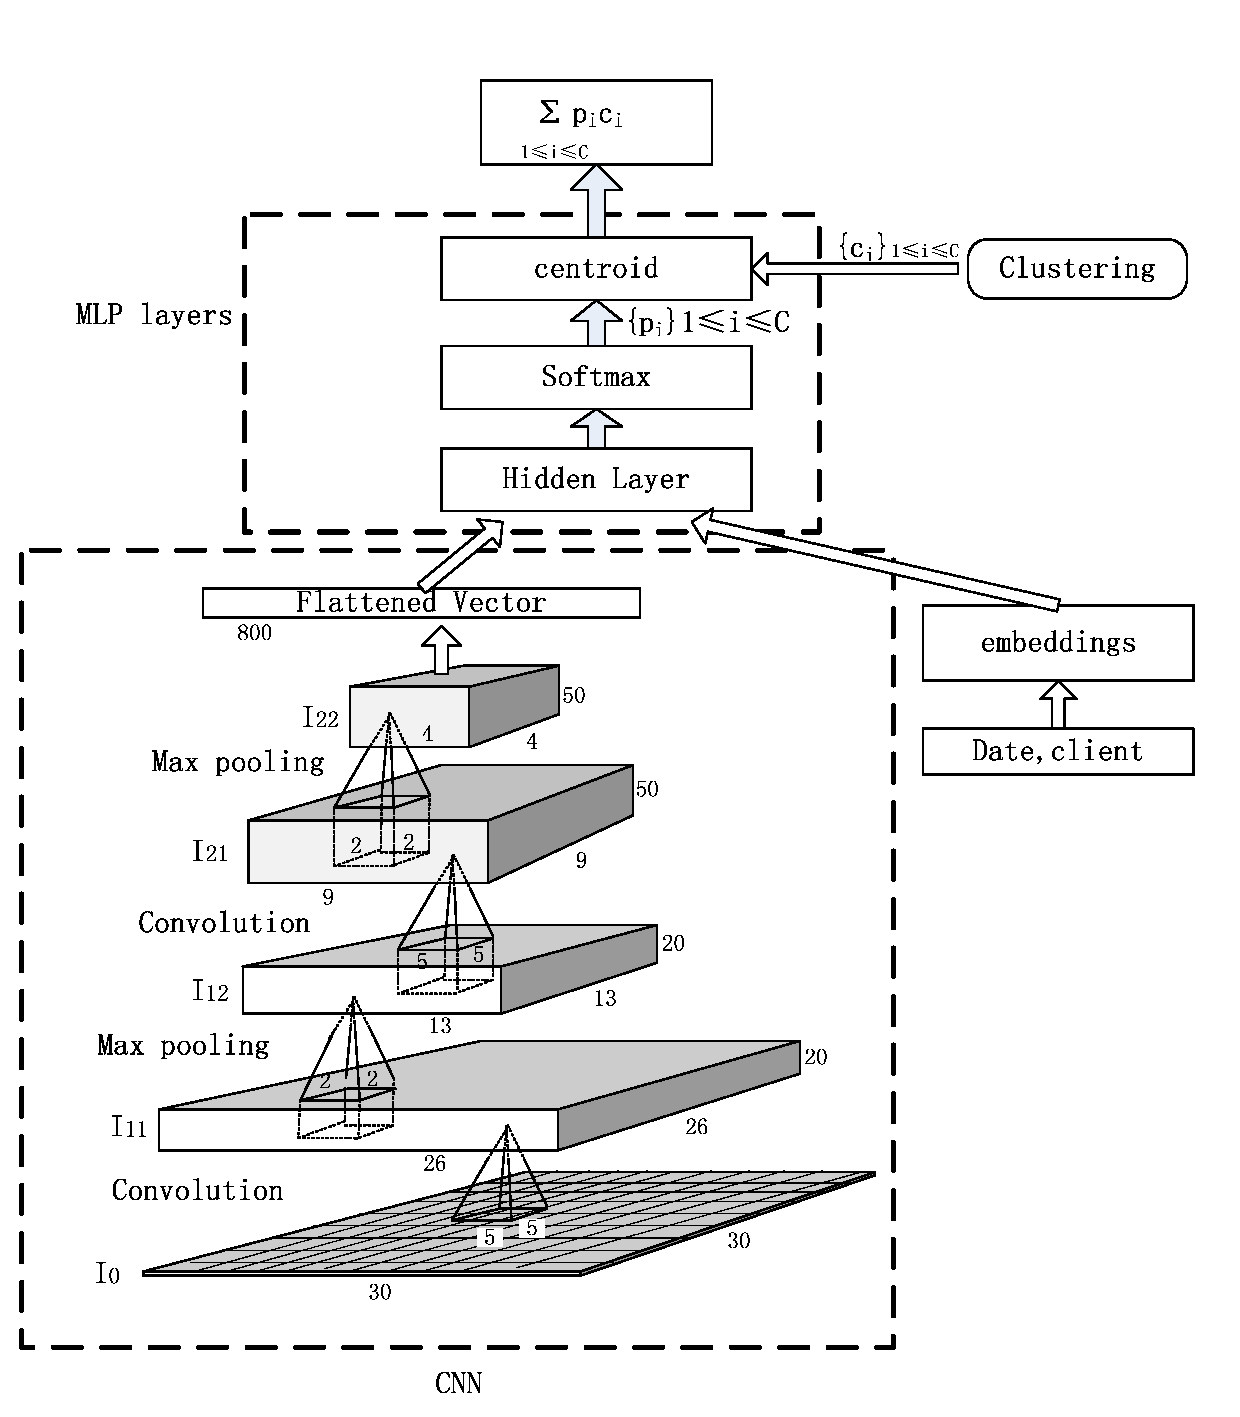
\includegraphics[width=1\textwidth]{./fig/cnn-new.pdf}
\end{minipage}
}
\caption{Architecture of T-CONV-global}
\label{T-CONV-global}
\end{figure}

The output  features of the top CNN layer are flattened into one-dimensional series and fed to the MLP layers, which is exactly the same as the champion model \cite{de2015artificial} of the ECML-PKDD competition \cite{kaggle2015}. Specifically,  the predicted destination is calculated as the weighted average of  the  cluster centers$\{c_i\}$, which are calculated by clustering the destinations of the historical trajectories \cite{de2015artificial}. The weight vector  $\{p_i\}$  is obtained by applying the softmax function to the  activation output  of the Hidden layer as follows:
 \begin{eqnarray}
p_i=\frac{exp(e_i)}{\sum_j{exp(e_j)}} \nonumber
 \end{eqnarray}

Here $(e_i)$ is an activation output of the hidden layer. Moreover, the meta data about date and client information, are also embedded as input vectors of the MLP layers. Readers can refer to the research  \cite{de2015artificial} for more detail about the MLP layers here. The fundamental difference between T-CONV and  \cite{de2015artificial} is that we utilize the CNN model to extract multi-scale trajectory patterns,  instead of using the raw spatial points as input of MLP.


 \begin{figure}
\centering
{
\begin{minipage}[b]{0.4\textwidth}
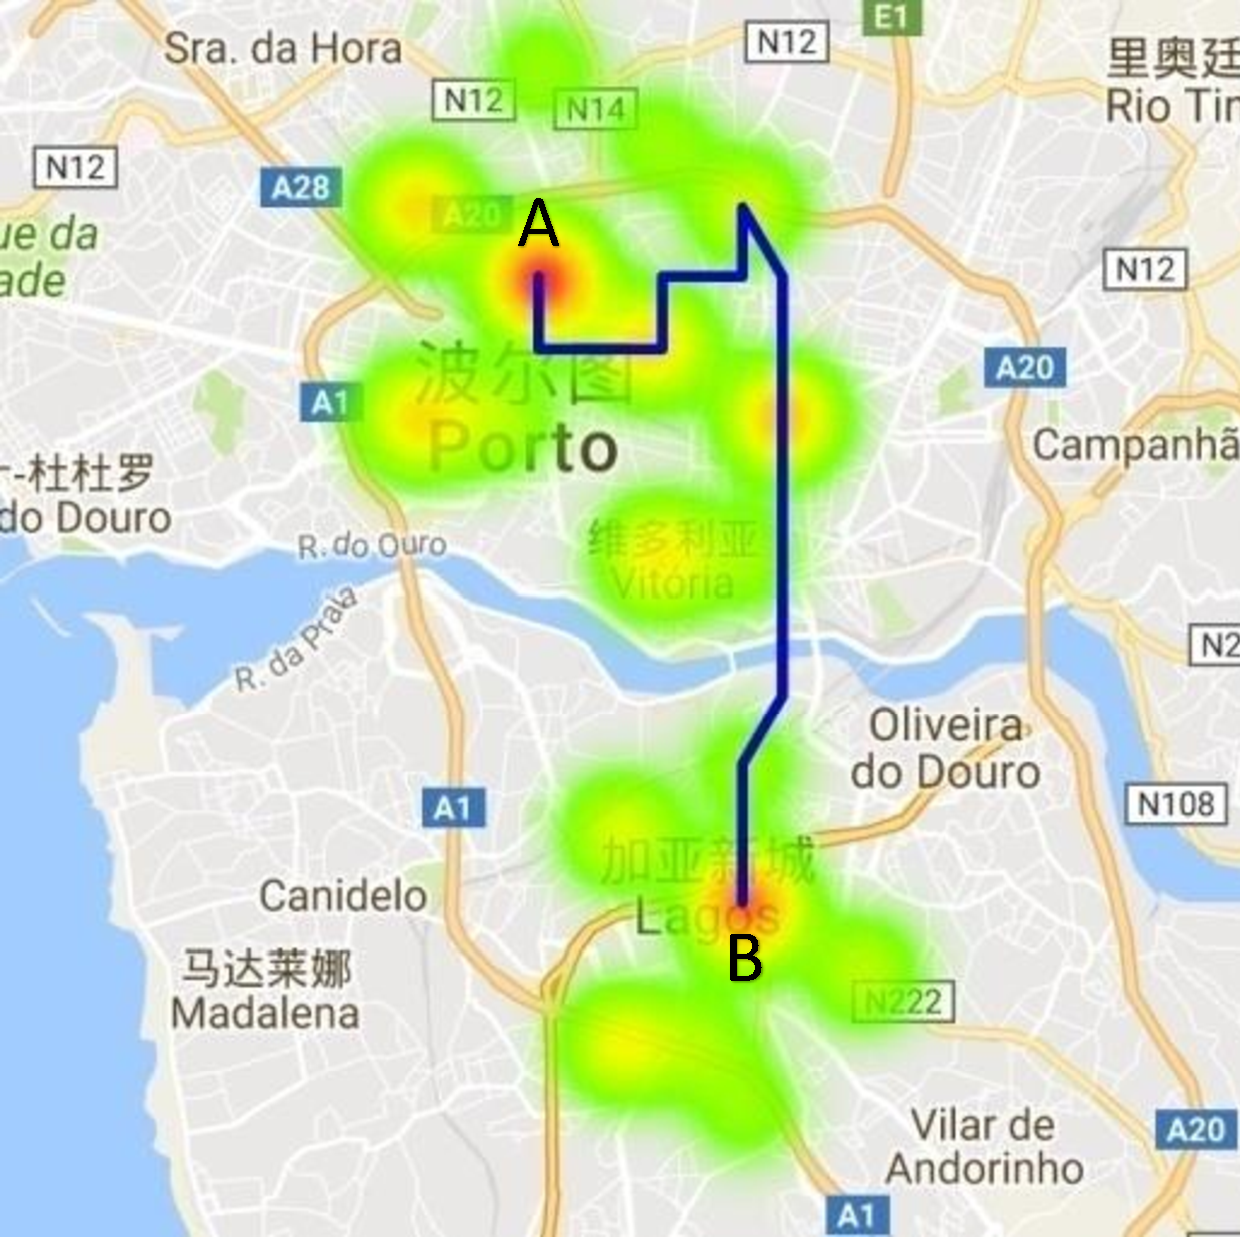
\includegraphics[width=1\textwidth]{./fig/Doc10.pdf}
\end{minipage}
}
\caption{The pattern captured in the layer $L_{22}$ of T-CONV-global. The orientation point of the trajectory is the 'A' point and the end point is 'B'.}
\label{L22}
\end{figure}

\begin{figure}
\centering
{
\begin{minipage}[b]{0.4\textwidth}
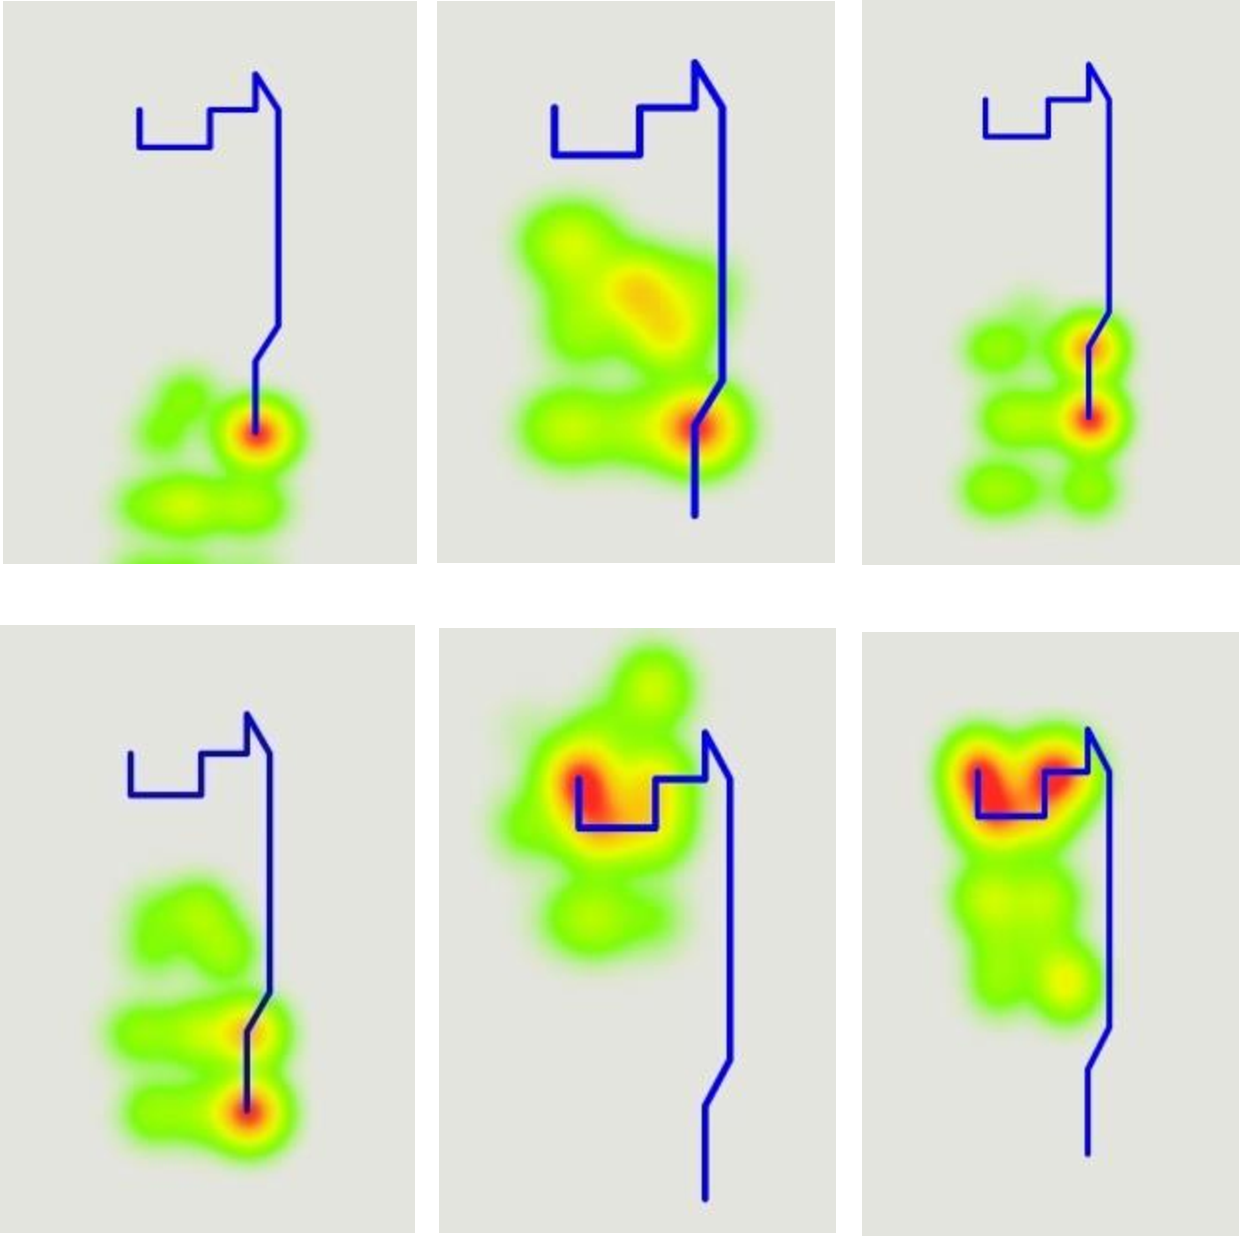
\includegraphics[width=1\textwidth]{./fig/Doc11.pdf}
\end{minipage}
}
\caption{The pattern captured in the layer $L_{12}$ of T-CONV-global.}
\label{L12}
\end{figure}

\subsection{Visualization of Learned Features}

In order to analyze the multi-scale patterns extracted from the T-CONV-global model clearly, we utilize the deconvolution methods introduced in \cite{zeiler2014visualizing} to visualize the patterns captured in different levels of the model, after training the model with the trajectory set  from the ECML-PKDD competition\cite{kaggle2015}.
The deconvolution method \cite{zeiler2014visualizing} uses a feature of any max-pooling layer as input, and adopts unpooling and deconvolution operations to recover the patterns, which are captured by this feature in the original trajectory image.

Fig.~\ref{L22}  shows the patterns captured by the layer $I_{22}$ of  T-CONV-global, while processing a trajectory. The patterns are generated by selecting the largest feature in $I_{22}$, which has the greatest impact  on the prediction result, and using the deconvolution method to  recover the information on the original trajectory image. In a similar way, as showed in Fig.~\ref{L12}, we select the top 6 features of the layer $I_{12}$ and visualize the patterns captured by them. Fig.~\ref{L12}  shows that the layer $I_{12}$ can capture the small-scale patterns, which focus on the details of the local changing in small local areas. Meanwhile, Fig.~\ref{L22}  shows that the higher layer $I_{22}$ can combine the lower level small-scale patterns  into effective patterns in larger scale.



Furthermore, the red and thick areas in Fig.~\ref{L22} and Fig.~\ref{L12}  are corresponding to bigger values and indicate  important portions in the patterns. From Fig.~\ref{L22}, it is interesting to find that the trained T-CONV model can recognize that the local areas close to the orientation point and end point of the trajectory contribute much more to the destination prediction. Intuitively, the end part of the trajectories is important, because it is closest to the destination and shows the direction and the trend of the  trajectories most recently.  Meanwhile, the sub-trajectory near the orientation is also important, while it indicates where the customer comes from and represents some inner motivation of the trip.  This observation motivates us to design some prediction models  focusing these two important local areas to improve the training efficiency.



\subsection{Local CNN with Multiple Spatial Channels}
As mentioned in the recent research\cite{xue2013destination,xue2015solving}, the sparsity problem of trajectories is ubiquitous and can have serious side-effects on the prediction accuracy.  Fig.~\ref{sparsity} illustrates the sparsity of the real trajectory dataset from the ECML-PKDD competition\cite{kaggle2015}, which contains about 1.7 million of trajectories. We divide the map into 30*30 grids and represent each trajectory as one sequence of cell IDs.  Then we randomly select one trajectory from the dataset, take its sub-trajectory with different length, and test the number of overlapping trajectories in the dataset.  When the length of the query trajectory is increased to more than 3, the number of overlapping trajectories drops sharply. This validates that the overlap degree of long trajectories is relatively low, and they trend to have diverse motion patterns.  This make it hard to mine some common patterns of  long trajectories.

\begin{figure}
\centering
{
\begin{minipage}[b]{0.4\textwidth}
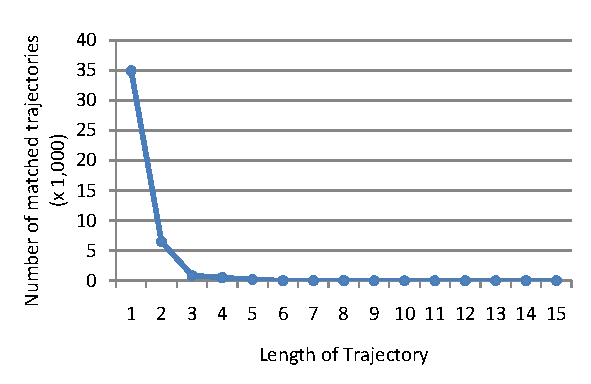
\includegraphics[width=1\textwidth]{./fig/Doc6.pdf}
\end{minipage}
}
\caption{Number of matched trajectories in the dataset VS the length of the query trajectory.}
\label{sparsity}
\end{figure}

On the other hand, as observed from the visualization of the T-CONV-global model in the last section, the areas close to the start and end of a trajectory have much more important contribution to the destination prediction than other areas. If we apply convolution only on these important local zones, instead of the global image,  the overlay degree of the short sub-trajectories can be much higher than that of global trajectories. The sparsity problem can be overcome, and it may be easier to capture common motion patterns.

Based on above analysis, we present the model \textbf{T-CONV-local} as illustrated in  Fig.~\ref{T-CONV-local}. T-CONV-local focuses on the two local zones centered at the start and the end of the input trajectory, while neglecting other parts.  Each local zone is then divided into a $M*M$ grid. In order to maintain the position information of the local zones, the accurate latitude and longitude of each cell is embedded into the two images: \emph{latitude image} $I_a$  and \emph{longitude image} $I_o$.  Given any taxi trajectory $T_k = \{P_{k1},P_{k2},...,P_{kt}\}$, the value of each pixel in $I_a$  is assigned as follows:
\begin{figure}
\centering
{
\begin{minipage}[b]{0.4\textwidth}
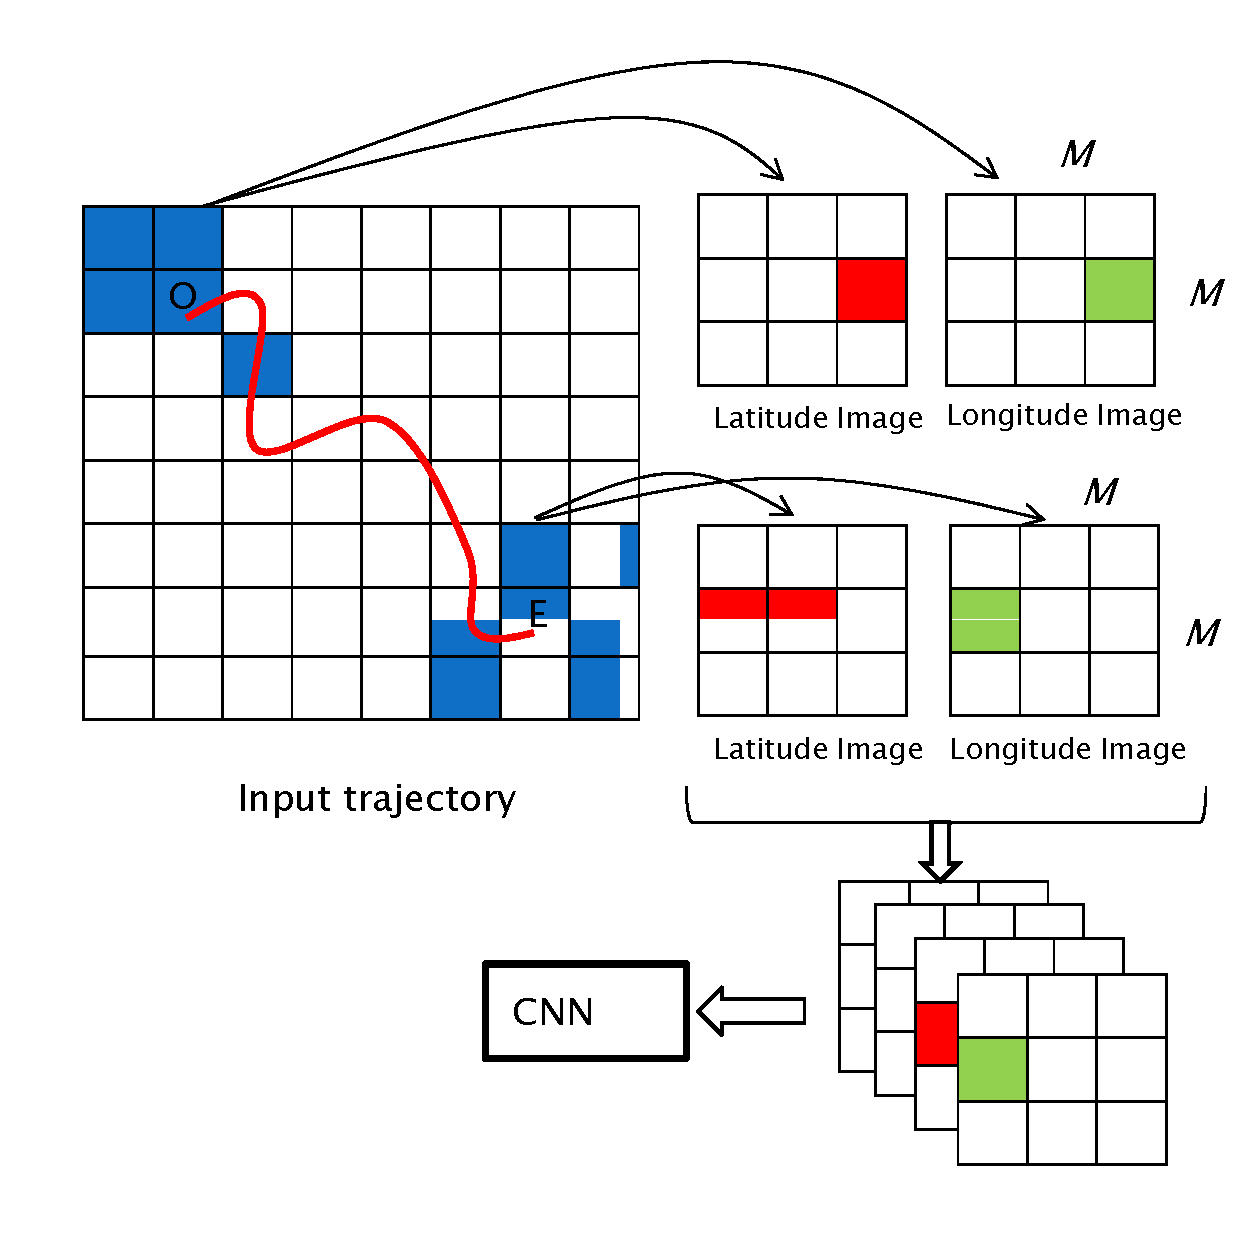
\includegraphics[width=1\textwidth]{./fig/Doc5.pdf}
\end{minipage}
}
\caption{Architecture of T-CONV-local}
\label{T-CONV-local}
\end{figure}



\[I_{a}(m,n)=\begin{cases}
f(Lat(C_{mn}))&\text{if  $\exists i (1 \leq i \leq t \wedge P_{ki} \in C_{mn})$}\\
0&\text{otherwise}
\end{cases}\]
The value of each pixel in $I_o$  is assigned as follows:

\[I_{o}(m,n)=\begin{cases}
g(Lon(C_{mn}))&\text{if $\exists i (1 \leq i \leq t \wedge P_{ki} \in C_{mn})$}\\
0&\text{otherwise}
\end{cases}\]

Here $Lat(C_{mn})$ means the latitude of the center of the cell $C_{mn}$, while $Lon(C_{ij})$ means the longitude of the same position. $f(.)$ and $g(.)$ are normalization function to transform their input into the range [-1,1]. Based on above processing, totally 4 images indicating different spatial channels can be obtained, which are stacked together and fed to the convolutional neural network of Fig.~2.

By replacing the global convolution with the local convolution operations on important local areas, the sparsity degree can be reduced to benefit better extraction of important patterns. Furthermore, while only focusing on small subsets of the whole image, the computation complexity of T-CONV-local can be much lower than T-CONV-global, given a same spatial scale.

\doublerulesep 0.1pt
\begin{table}[h]
\centering
\begin{footnotesize}
\caption{The evaluation errors of different models} \label{tab:notation}
\begin{tabular}{p{4.5cm} p{1.5cm}}
\hline\hline\noalign{\smallskip}
    \textbf{Model} & \textbf{error}  \\
\hline\hline
    MLP & 2.81 \\
\hline\hline
    Bidirectional RNN & 3.01 \\
\hline\hline
    Bidirectional RNN with window & 2.60 \\
\hline\hline
    Memory network  & 2.87 \\
\hline\hline
    \textbf{T-CONV-global} & \textbf{2.73} \\
\hline\hline
    \textbf{T-CONV-local} & \textbf{2.53} \\
\hline\hline


\end{tabular}
\end{footnotesize}
\end{table}

\section{Evaluation}
In this section, we conduct comprehensive experiments to validate the effectiveness of the T-CONV models, and compare with the other state-of-the-art algorithms.

\subsection{Experiment Setup}

We test the performance of T-CONV on the real trajectory dataset of the ECML-PKDD competition\cite{kaggle2015}, which  is collected from 442 taxis running in the city of Porto for a complete year (from 2013-07-01 to 2014-06-30), and has totally 1.7 millions complete trajectories.  In order to validate the prediction accuracy, we use the same testing dataset as\cite{de2015artificial}, which  contains 19,770 incomplete trajectories randomly selected from the original dataset.  The remaining trajectories are used for training.

In this paper, we mainly compare T-CONV with the neural networks based models\cite{de2015artificial}, which win the champion of  the ECML-PKDD competition\cite{kaggle2015}. These models are listed as follows:

\begin{itemize}
\item \emph{MLP} : a multi-layer perceptron model like the MLP layers in the Fig.~2. The inputs of the models are the latitudes and longitudes of the first and last 5 points in the  trajectory.

\item \emph{Bidirectional RNN}: a bidirectional recurrent neural network, which considers a trajectory as a sequence and  each GPS point in the trajectory forms a transition state of RNN.

\item \emph{Bidirectional RNN with window}: a variant of the above Bidirectional RNN model, which uses a sliding window of 5 successive GPS points as a transition state of RNN.

\item \emph{Memory network}: a variant of the above RNN model, which encodes  trajectories into vectors with fixed length, and compares the similarity between the input trajectories and historical trajectories in this vector space.
\end{itemize}

The evaluation error of the models is defined as the Haversine distance between the real destination and the predicted location as follows:

 \begin{eqnarray}
   d(x,y) &=& 2 \cdot r \cdot \arctan (\sqrt{\frac{a}{1-a}}) \nonumber
\end{eqnarray}
where
 \begin{eqnarray}
   a = \sin^{2}(\frac{\phi_x - \phi_y}{2})+\cos��\phi_x��\cos��\phi_y��\sin^{2}(\frac{\lambda_x - \lambda_y}{2}) \nonumber
\end{eqnarray}
Here $\phi$ indicates the latitude  and $\lambda$ indicates the longitude. r  is the radius of the earth.

\subsection{Performance}

The prediction errors of our proposed models are compared with other baseline models in the Table 1.   The result shows that both T-CONV models are much better than the  MLP model. As illustrated in Fig.~2 T-CONV models share similar output layers as the MLP layers, but use the multi-layer  CNN to capture multi-scale  trajectory patterns. The much better performance of T-CONV indicates that the effectiveness of  the multi-scale patterns extracted by CNN.  In Addition, the T-CONV model is also better than the Bidirectional RNN model and Memory network, which are also based on one single spatial scale.

While looking into the two T-CONV models, T-CONV-local is much better than T-CONV-global. This shows that the convolution on the important local areas can enhance the ability of CNN to capture significant patterns. As showed in Fig.~\ref{ratio}, we also test the prediction performance of these two models given the trajectories with different completeness ratio. The complete ratio indicates the percentage of the current observed trajectory compared to its  full trajectory, and it implies how far the end point of the trajectory is from the destination. Fig.~\ref{ratio} shows that  when a taxi is  closer to the destination, lower prediction error can be achieved. Furthermore, it also shows that T-CONV-local shows smaller error in most of the cases.


\begin{figure}
\centering
{
\begin{minipage}[b]{0.4\textwidth}
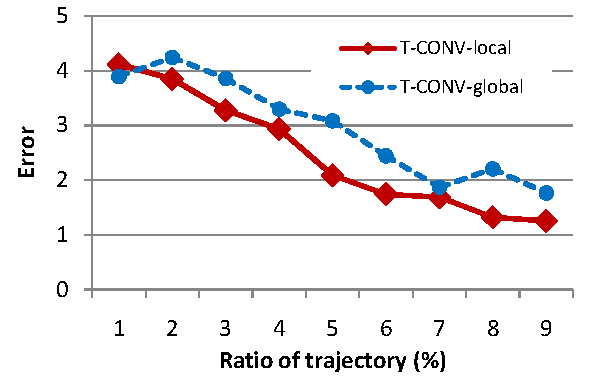
\includegraphics[width=1\textwidth]{./fig/Doc7.pdf}
\end{minipage}
}
\caption{The prediction error given different completeness ratio of trajectories }
\label{ratio}
\end{figure}

\subsection{Sensibility of Parameters}

In this section, we test that how the change of hyper parameters of T-CONV-local affects its prediction accuracy.  We focus on the following two parameters directly related to the spatial scale to process  trajectories:

 \begin{itemize}
 \item $M$: As illustrated in Fig.~\ref{T-CONV-local}, $M$ is the number of rows (or columns) of the grid. Higher $M$ is corresponding to a denser grid.
\item $W$: $W$ denotes the width of each cell in meters.  Thus $M*W$ indicates the width of the local areas of T-CONV-local. Given any fixed configuration of $M$, larger $W$ means  that larger portions of the trajectories are input into the model.
 \end{itemize}

We test the performance of  T-CONV-local  with different combinations of  $M$ and $W$. Fig.~\ref{differentWM}shows how the prediction error decreases along with the training iterations. Specifically, Fig.~\ref{differentWM}(a) shows the performance of  the models with different $W$ while  keep $M$ unchanged, and Fig.~\ref{differentWM}(b) shows the performance of this model  with different $M$ given fixed $W$.  In these experiments, the other hyper parameters are assigned  as the values showed in Fig.~\ref{T-CONV-global}. Fig.~\ref{differentWM} indicates that the performance of T-CONV-local is not sensible to the slight changing of $M$ and $W$. That means although $M$ and $W$ affect the scale of the input trajectory image, the multi-layer convolutional neural networks of T-CONV are robust to extract multi-scale patterns for precise prediction.

\begin{figure}
\centering
\subfigure[]{
\begin{minipage}[b]{0.4\textwidth}
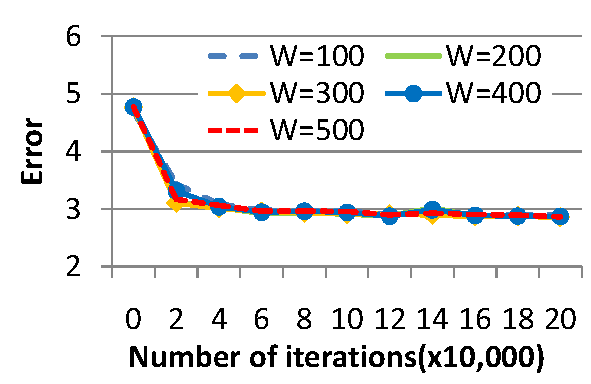
\includegraphics[width=1\textwidth]{./fig/Doc8.pdf}
\end{minipage}
}
\subfigure[]{
\begin{minipage}[b]{0.4\textwidth}
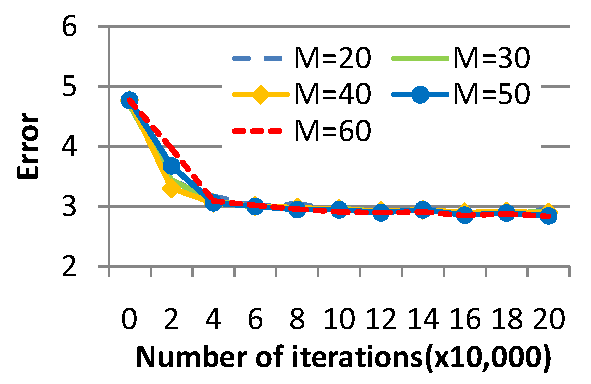
\includegraphics[width=1\textwidth]{./fig/Doc9.pdf}
\end{minipage}
}
\caption{ The prediction error of  T-CONV-local with different $W$ and $M$.
(a) T-CONV-local with different $W$, $M$ is kept fixed as 30 here.
(b) T-CONV-local with different $M$. Here $W$ is kept fixed as 100.
 }
 \label{differentWM}
\end{figure}


\section{ Conclusions}
In this paper, we present the convolutional neural network based model, T-CONV, to predict the destinations of taxi trajectories. Different from traditional research which models trajectories as one-dimensional sequences in one single scale, T-CONV models trajectories as two-dimensional images and  combines multi-scale trajectory patterns through multi-layer convolution operations to achieve better prediction accuracy. Specifically, the effectiveness of the T-CONV-local model shows that the multiple local convolutional fields focusing on important local areas can perform much better than the T-CONV-global model which conducts convolution over the whole trajectory image.


\bibliographystyle{aaai}
\bibliography{Ref}
\end{document}
